\documentclass[compress,12pt]{beamer}

\usetheme{Arguelles}

\usepackage{markup}
\usepackage{listings}
\usepackage{juliamono}
\usepackage{unicode-math}
\usepackage{graphicx}
\usepackage{subcaption}
\usepackage{tikz-3dplot}
\usepackage[autostyle, style=english]{csquotes}
\usetikzlibrary{automata, positioning, arrows, arrows.meta, tikzmark, shapes.geometric, hobby, patterns, shapes.multipart, decorations.pathmorphing, graphdrawing, graphs, chains, calligraphy, snakes}

\setmathfont{Erewhon-Math.otf}[CharacterVariant={20}]
\renewcommand{\mathsf}[1]{\textup{\textsf{#1}}}
\let\mathds\mathbb

\lstset{
  basicstyle=\ttfamily,
  captionpos=b,
}

\MakeOuterQuote{"}

\usepackage{xcolor}

\definecolor{rp-dark-base}{HTML}{191724}
\definecolor{rp-dark-surface}{HTML}{1F1D2E}
\definecolor{rp-dark-overlay}{HTML}{26233A}
\definecolor{rp-dark-muted}{HTML}{6E6A86}
\definecolor{rp-dark-subtle}{HTML}{908CAA}
\definecolor{rp-dark-text}{HTML}{E0DEF4}
\definecolor{rp-dark-love}{HTML}{EB6F92}
\definecolor{rp-dark-gold}{HTML}{F6C177}
\definecolor{rp-dark-rose}{HTML}{EBBCBA}
\definecolor{rp-dark-pine}{HTML}{31748F}
\definecolor{rp-dark-foam}{HTML}{9CCFD8}
\definecolor{rp-dark-iris}{HTML}{C4A7E7}
\definecolor{rp-dark-highlight-low}{HTML}{21202E}
\definecolor{rp-dark-highlight-med}{HTML}{403D52}
\definecolor{rp-dark-highlight-high}{HTML}{524F67}

\definecolor{rp-light-base}{HTML}{FAF4ED}
\definecolor{rp-light-surface}{HTML}{FFFaf3}
\definecolor{rp-light-overlay}{HTML}{F2E9E1}
\definecolor{rp-light-muted}{HTML}{9893A5}
\definecolor{rp-light-subtle}{HTML}{797593}
\definecolor{rp-light-text}{HTML}{575279}
\definecolor{rp-light-love}{HTML}{B4637A}
\definecolor{rp-light-gold}{HTML}{EA9D34}
\definecolor{rp-light-rose}{HTML}{D7827E}
\definecolor{rp-light-pine}{HTML}{286983}
\definecolor{rp-light-foam}{HTML}{56949F}
\definecolor{rp-light-iris}{HTML}{907AA9}
\definecolor{rp-light-highlight-low}{HTML}{F4EDE8}
\definecolor{rp-light-highlight-med}{HTML}{DFDAD9}
\definecolor{rp-light-highlight-high}{HTML}{CECBCD}

\title{Curved Point-Normal Triangles.}
\author{Hugo SALOU}

\begin{document}
  \frame[plain]{\titlepage}

  \Section{PN Triangles}

  \begin{frame}
    \frametitle{Point-Normal triangle.}
    \centering
    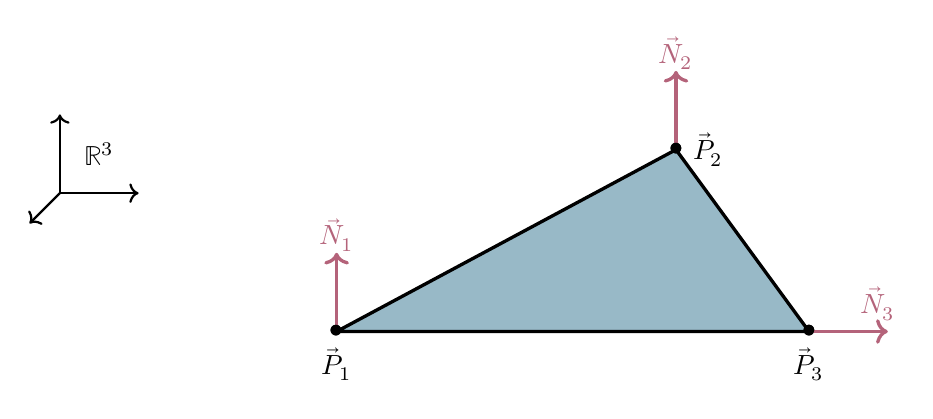
\begin{tikzpicture}
      \filldraw[fill=rp-dark-pine!50,very thick] (0, 0, 0) -- (2, 0, -6) -- (6, 0, 0) -- (0, 0, 0);

      \begin{scope}[xshift=-100,yshift=50,thick]
        \draw[->] (0, 0, 0) -- (1, 0, 0);
        \draw[->] (0, 0, 0) -- (0, 1, 0);
        \draw[->] (0, 0, 0) -- (0, 0, 1);
        \node at (0.5, 0.5, 0) {$\mathds{R}^3$};
      \end{scope}

      \node[inner sep=0pt] (a) at (0, 0, 0)  {$\bullet$};
      \node[inner sep=0pt] (b) at (2, 0, -6) {$\bullet$};
      \node[inner sep=0pt] (c) at (6, 0, 0)  {$\bullet$};

      \node[below=0cm of a] {$\vec P_1$};
      \node[right=0cm of b] {$\vec P_2$};
      \node[below=0cm of c] {$\vec P_3$};

      \pause

      \draw[very thick, rp-light-love, ->] (0, 0, 0) to  node[above, very near end] {$\vec N_1$} +(0, 1, 0);
      \draw[very thick, rp-light-love, ->] (2, 0, -6) to node[above, very near end] {$\vec N_2$} +(0, 1, 0);
      \draw[very thick, rp-light-love, ->] (6, 0, 0) to  node[above, very near end] {$\vec N_3$} +(1, 0, 0);

      \node[inner sep=0pt] (a) at (0, 0, 0)  {$\bullet$};
      \node[inner sep=0pt] (b) at (2, 0, -6) {$\bullet$};
      \node[inner sep=0pt] (c) at (6, 0, 0)  {$\bullet$};
    \end{tikzpicture}
    \begin{markups}
      \addmarkup<3>{annotations/point-normal-mesh.pdf}
    \end{markups}
  \end{frame}

  \begin{frame}
    \frametitle{\textit{Curved} PN triangle.}

    \centering
    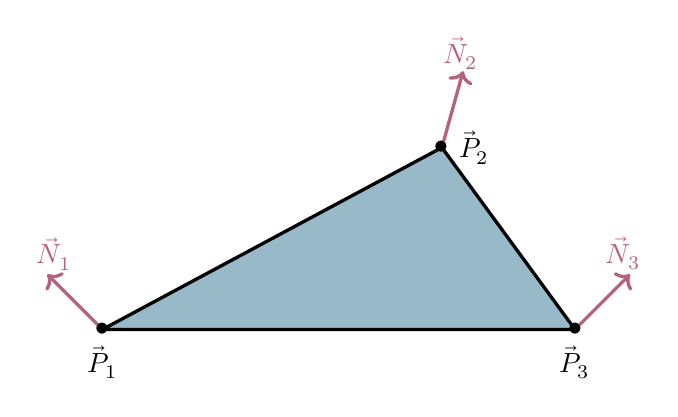
\begin{tikzpicture}
      \filldraw[fill=rp-dark-pine!50,very thick] (0, 0, 0) -- (2, 0, -6) -- (6, 0, 0) -- (0, 0, 0);

      \node[inner sep=0pt] (a) at (0, 0, 0)  {$\bullet$};
      \node[inner sep=0pt] (b) at (2, 0, -6) {$\bullet$};
      \node[inner sep=0pt] (c) at (6, 0, 0)  {$\bullet$};

      \node[below=0cm of a] {$\vec P_1$};
      \node[right=0cm of b] {$\vec P_2$};
      \node[below=0cm of c] {$\vec P_3$};

      \draw[very thick, rp-light-love, ->] (0, 0, 0) to  node[above, very near end] {$\vec N_1$} +(-0.7, 0.7, 0);
      \draw[very thick, rp-light-love, ->] (2, 0, -6) to node[above, very near end] {$\vec N_2$} +(0, 0.7, -0.7);
      \draw[very thick, rp-light-love, ->] (6, 0, 0) to  node[above, very near end] {$\vec N_3$} +(0.7, 0.7, 0);

      \node[inner sep=0pt] (a) at (0, 0, 0)  {$\bullet$};
      \node[inner sep=0pt] (b) at (2, 0, -6) {$\bullet$};
      \node[inner sep=0pt] (c) at (6, 0, 0)  {$\bullet$};
    \end{tikzpicture}
    \begin{markups}
      \addmarkup<2>{annotations/bezier-patch.pdf}
    \end{markups}
  \end{frame}
  
  \begin{frame}
    \frametitle{An explicit formula.}
    \[
      \begin{array}{r|rcl}
        \vec b:& \Delta &\longrightarrow &\mathds{R}^3 \\
               &(u,v, w)&\longmapsto& \sum_{i+j+k=3} \vec b_{kij} \: u^i v^j w^k
      ,\end{array}
    \] 
    \begin{align*}
      \vec{b}_{300} &:= \vec{P}_1, & 
      \vec{b}_{030} &:= \vec{P}_2, & 
      \vec{b}_{003} &:= \vec{P}_3, &
      w_{ij} := ( \vec{P}_{j} - \vec{P}_{i} ) \cdot \vec{N}_{i}
    \end{align*}
    \vspace{-\baselineskip}
    \begin{align*}
      \vec{b}_{012} &:= \frac{1}{3} ( 2 \vec{P}_{3} + \vec{P}_{2} - w_{32}\vec{N}_{3}), &
      \vec{b}_{021} &:= \frac{1}{3} ( 2 \vec{P}_{2} + \vec{P}_{3} - w_{23}\vec{N}_{2}), &&\\
      \vec{b}_{102} &:= \frac{1}{3} ( 2 \vec{P}_{3} + \vec{P}_{1} - w_{31}\vec{N}_{3}), &
      \vec{b}_{201} &:= \frac{1}{3} ( 2 \vec{P}_{1} + \vec{P}_{3} - w_{13}\vec{N}_{1}), &&\\
      \vec{b}_{120} &:= \frac{1}{3} ( 2 \vec{P}_{2} + \vec{P}_{1} - w_{21}\vec{N}_{2}), &
      \vec{b}_{210} &:= \frac{1}{3} ( 2 \vec{P}_{1} + \vec{P}_{2} - w_{12}\vec{N}_{1}), &
    \end{align*}
    \vspace{-1\baselineskip}
    \begin{align*}
      \vec{b}_{111} &:= \alpha \vec{E} + (1 - \alpha) \vec{V} & 
      \vec{V} &:= \frac{1}{3} (\vec{P}_{1} + \vec{P}_{2}+ \vec{P}_{3})
    \end{align*}
    \vspace{-1\baselineskip}
    \begin{align*}
      \vec{E} &:= \frac{1}{6} (\vec{b}_{012} + \vec{b}_{021} + \vec{b}_{102} + \vec{b}_{201} + \vec{b}_{120} + \vec{b}_{210})
    .\end{align*}

    \begin{markups}
      \addmarkup<2>{annotations/control-points.pdf}
    \end{markups}
  \end{frame}

  \begin{frame}
    \frametitle{A few examples.}
    \framesubtitle{\itshape\bfseries\sffamily demo}

    
\includegraphics[width=0.25\paperwidth]{figures/suzanne-base.png}
    \hfill
    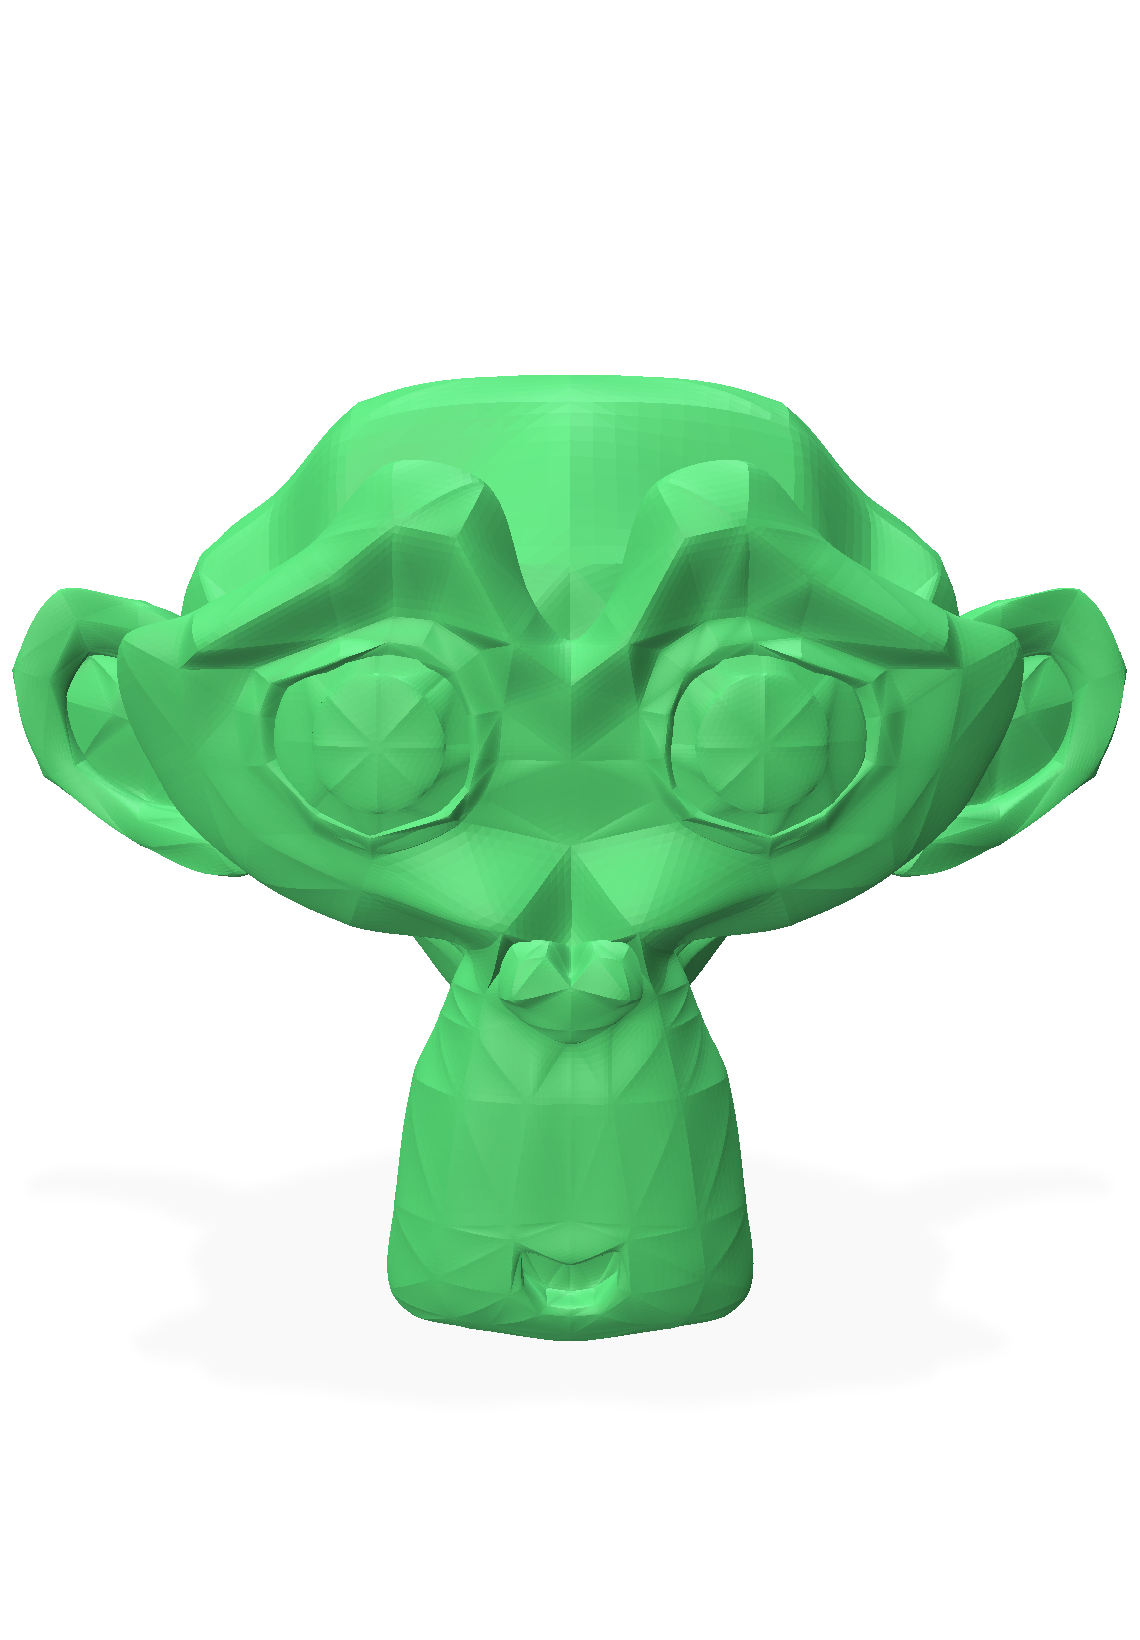
\includegraphics[width=0.25\paperwidth]{figures/suzanne-controls.png}
    \hfill
    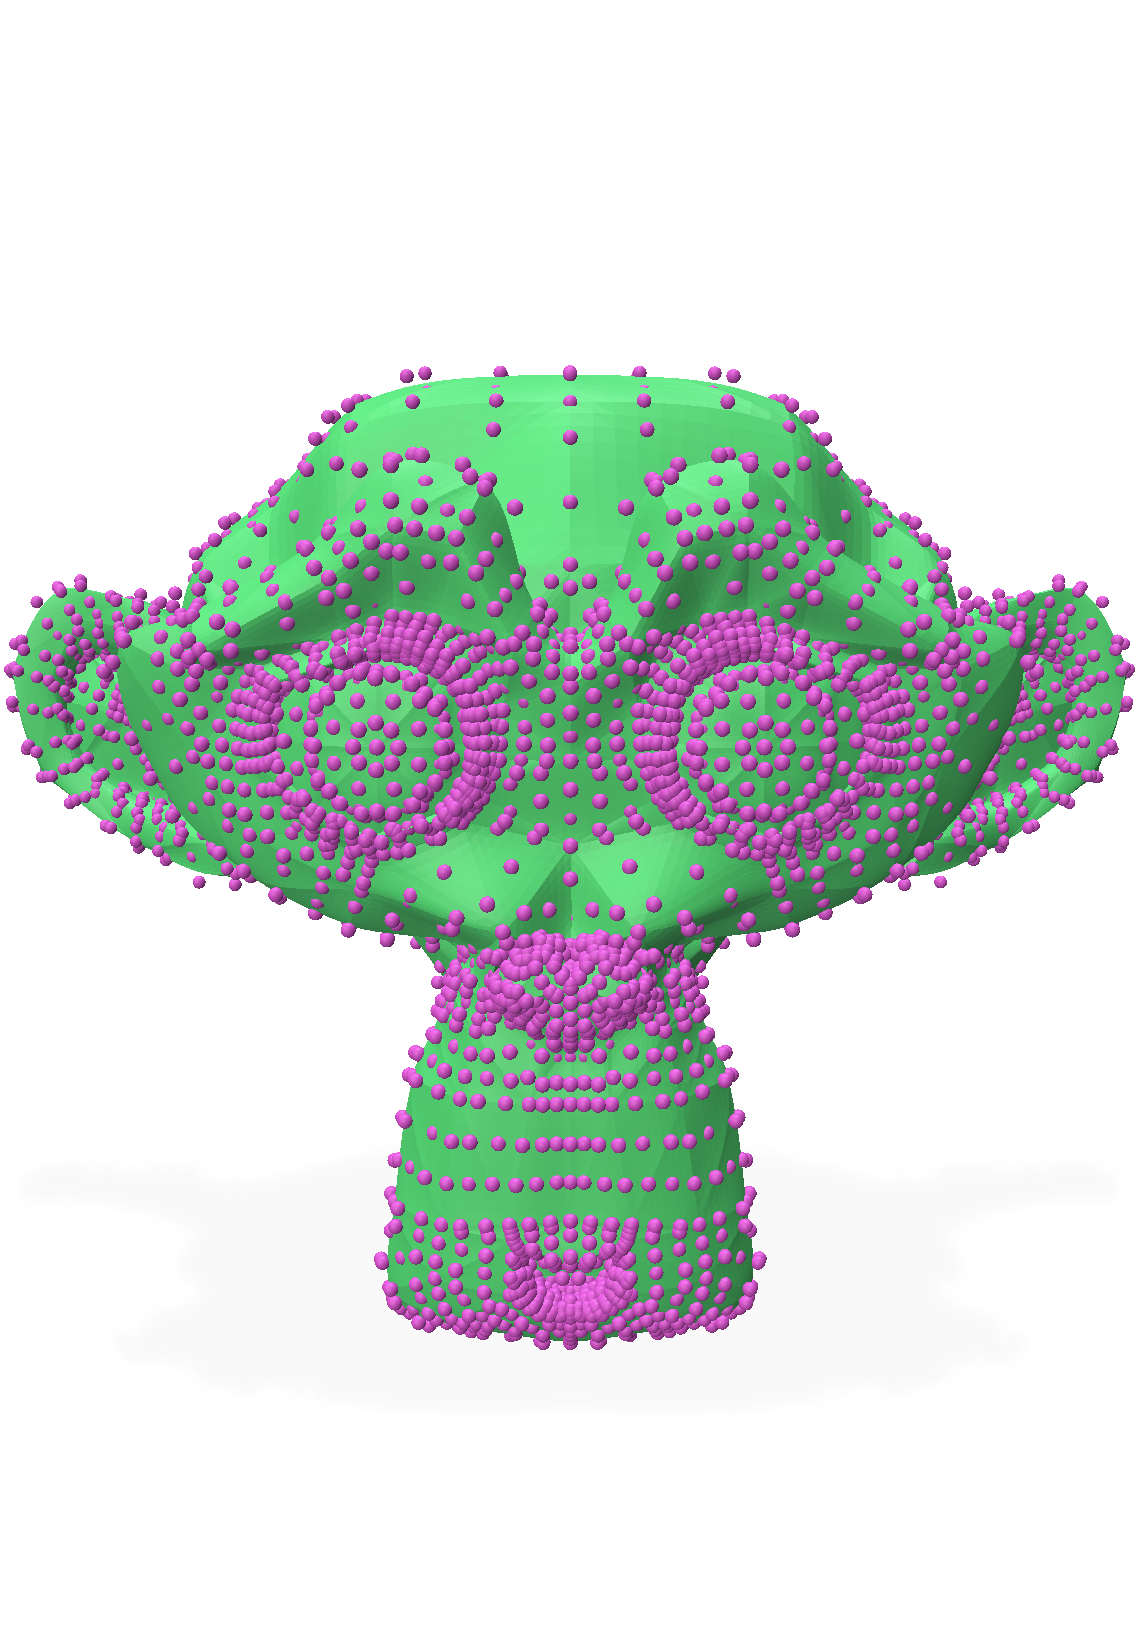
\includegraphics[width=0.25\paperwidth]{figures/suzanne-smooth.png}

    \begin{center}
      \texttt{python3 object.py data/suzanne-500.ply}
    \end{center}
  \end{frame}

  \Section{Normals}

  \begin{frame}
    \frametitle{Computing the normals: linear model.}

    \[
      \vec n(u, v, w) := \mathsf{normalized}\big( w \vec N_1 + u \vec N_2 + v \vec N_3 \big)
    \]
    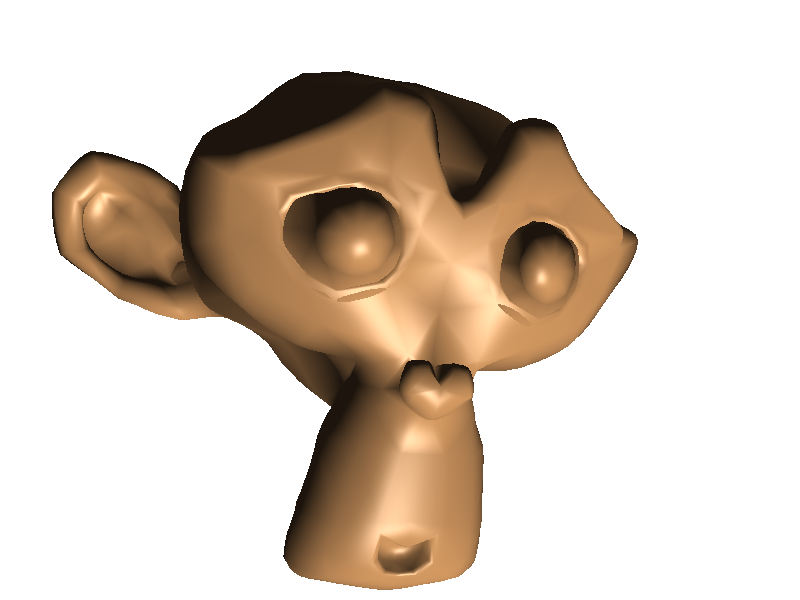
\includegraphics[width=0.5\textwidth]{figures/normals1.png}
  \end{frame}

  \begin{frame}
    \frametitle{Computing the normals: quadratic model.}

    \[
      \vec n(u, v, w) := \mathsf{normalized}\Big(\sum_{i+j+k = 2} \vec n_{kij} u^i v^j w^k\Big)
    \]
    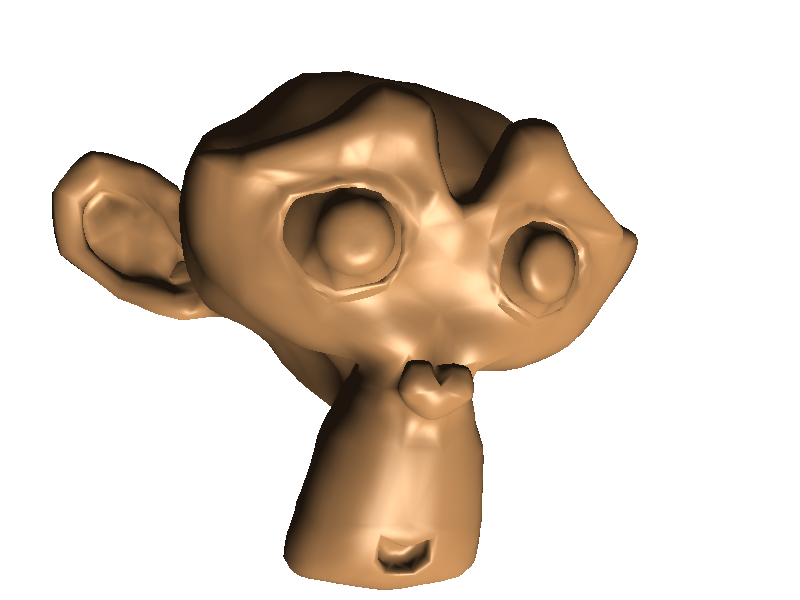
\includegraphics[width=0.5\textwidth]{figures/normals2.png}
  \end{frame}

  \begin{frame}
    \frametitle{Computing the normals: "exact" model.}

    \[
      \vec n(u, v, w) := \mathsf{normalized}\left( \frac{\partial \vec b(u,v,w)}{\partial u} \times \frac{\partial \vec b(u, v,w)}{\partial v} \right) 
    \]

    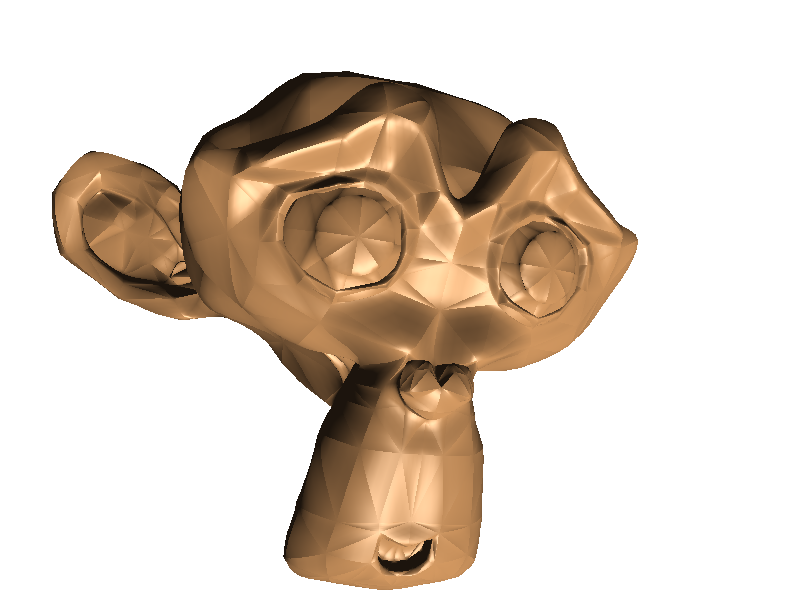
\includegraphics[width=0.5\textwidth]{figures/normals3.png}
  \end{frame}

  \begin{frame}
    \frametitle{Comparing the models.}

    \begin{figure}[htbp]
      \centering
      \subcaptionbox{Linear varying normals}{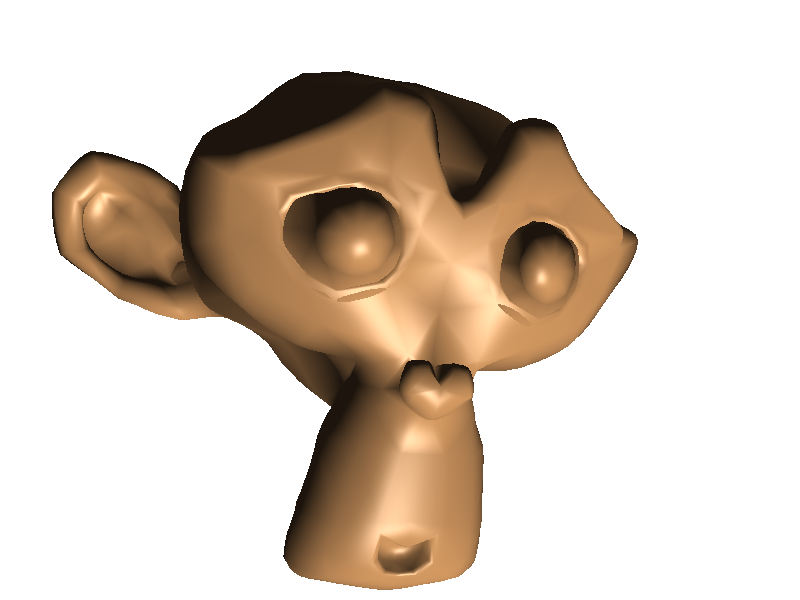
\includegraphics[width=0.25\paperwidth]{figures/normals1.png}}
      \subcaptionbox{Quadratic varying normals}{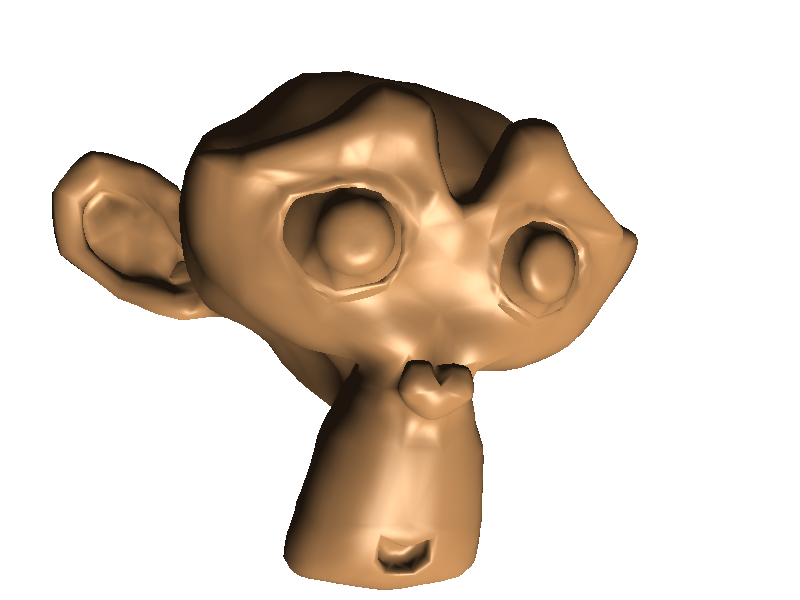
\includegraphics[width=0.25\paperwidth]{figures/normals2.png}}
      \subcaptionbox{"Exact" normals}{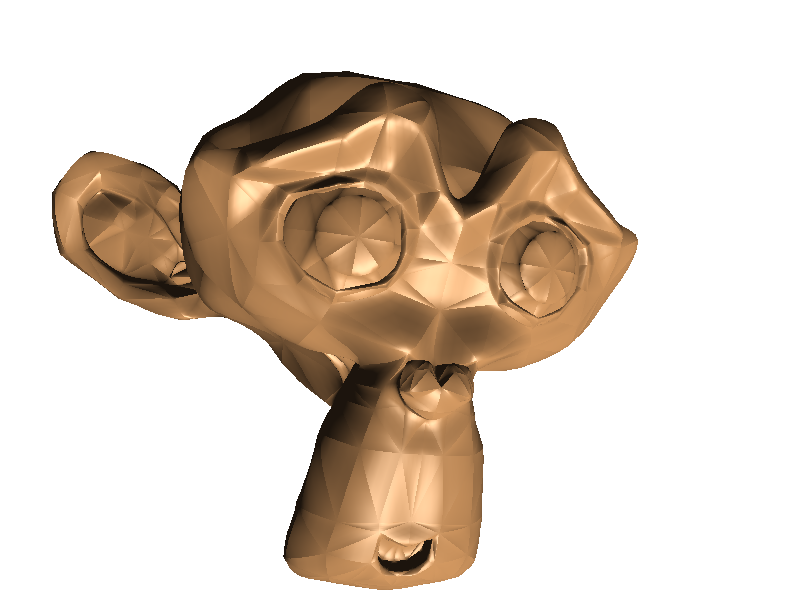
\includegraphics[width=0.25\paperwidth]{figures/normals3.png}}
      \caption{Comparison of different normals-computing methods}
    \end{figure}
  \end{frame}

  \Section{OpenGL}

  \begin{frame}
    \frametitle{The OpenGL Pipeline {\footnotesize\itshape (simplified)}.}

    \centering
    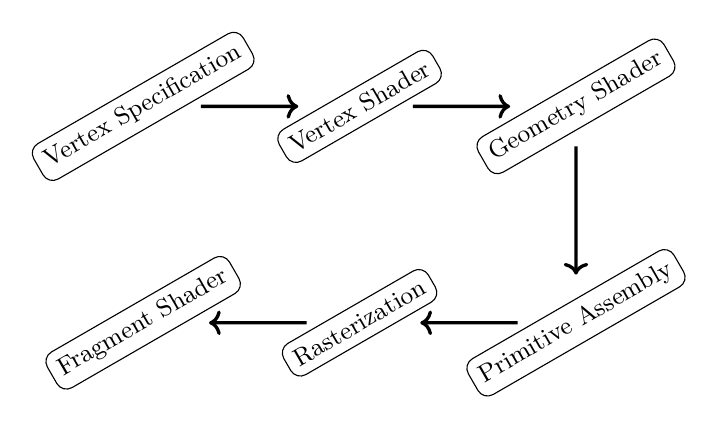
\begin{tikzpicture}[box/.style={draw,rectangle,rotate=30,rounded corners,minimum height=0.4cm,text centered}, shorten >=0.3cm,shorten <=0.2cm, font=\small]
      \node(a) {};
      \node[right=2.5cm of a] (b) {};
      \node[right=2.5cm of b] (c) {};
      \node[below=2.5cm of c] (d) {};
      \node[left=2.5cm of d] (e) {};
      \node[left=2.5cm of e] (f) {};
      \node[box] (va) at (a) {Vertex Specification};
      \node[box] (vb) at (b) {Vertex Shader};
      \node[box] (vc) at (c) {Geometry Shader};
      \node[box] (vd) at (d) {Primitive Assembly};
      \node[box] (ve) at (e) {Rasterization};
      \node[box] (vf) at (f) {Fragment Shader};
      \draw[very thick, ->] (va) to (vb);
      \draw[very thick, ->] (vb) to (vc);
      \draw[very thick, ->] (vc) to (vd);
      \draw[very thick, ->] (vd) to (ve);
      \draw[very thick, ->] (ve) to (vf);
    \end{tikzpicture}

    \begin{markups}
      \addmarkup<2->{annotations/opengl-geom1.pdf}
      \addmarkup<3->{annotations/opengl-geom2.pdf}
      \addmarkup<4->{annotations/opengl-geom3.pdf}
    \end{markups}
  \end{frame}

  \begin{frame}
    \frametitle{A few examples.}
    \framesubtitle{\itshape\bfseries\sffamily demo}

    \begin{center}
      \texttt{python3 opengl\_object.py data/suzanne-500.ply}
    \end{center}
  \end{frame}

  \Section{Applications}

  \begin{frame}
    \frametitle{A cloth simulation.}
    \framesubtitle{\itshape\bfseries\sffamily demo}

    \begin{tikzpicture}
      \node[inner sep=0pt] (a) {$\bullet$};
      \node[right = 2cm of a, inner sep=0pt]  (b) {$\bullet$};
      \node[right = 2cm of b, inner sep=0pt]  (c) {$\bullet$};
      \node[below = 2cm of a, inner sep=0pt]  (d) {$\bullet$};
      \node[below = 2cm of b, inner sep=0pt]  (n) {$\bullet$};
      \node[below = 2cm of c, inner sep=0pt]  (e) {$\bullet$};
      \node[below = 2cm of d, inner sep=0pt]  (f) {$\bullet$};
      \node[below = 2cm of n, inner sep=0pt]  (g) {$\bullet$};
      \node[below = 2cm of e, inner sep=0pt]  (h) {$\bullet$};
      \fill[oc-gray-2] (a) rectangle (h);
      \draw[snake=coil,segment amplitude=3,segment length=3,line cap=round] (n) to node[near end] (an)  {} node[midway] (am)  {} (a);
      \draw[snake=coil,segment amplitude=3,segment length=3,line cap=round] (n) to node[near end] (bn)  {} node[midway] (bm)  {} (b);
      \draw[snake=coil,segment amplitude=3,segment length=3,line cap=round] (n) to node[near end] (cn)  {} node[midway] (cm)  {} (c);
      \draw[snake=coil,segment amplitude=3,segment length=3,line cap=round] (n) to node[near end] (dn)  {} node[midway] (dm)  {} (d);
      \draw[snake=coil,segment amplitude=3,segment length=3,line cap=round] (n) to node[near end] (en)  {} node[midway] (em)  {} (e);
      \draw[snake=coil,segment amplitude=3,segment length=3,line cap=round] (n) to node[near end] (fn)  {} node[midway] (fm)  {} (f);
      \draw[snake=coil,segment amplitude=3,segment length=3,line cap=round] (n) to node[near end] (gn)  {} node[midway] (gm)  {} (g);
      \draw[snake=coil,segment amplitude=3,segment length=3,line cap=round] (n) to node[near end] (hn)  {} node[midway] (hm)  {} (h);
      \node[below = 2cm of b,inner sep=0pt]  (n) {$\bullet$};

      \filldraw[oc-gray-0,decoration={random steps,segment length=2mm, amplitude=3}, decorate, line width=5pt] (am.center) -- (cm.center) -- (hm.center) -- (fm.center) -- (am.center) -- (b.center) -- (current bounding box.north west) -- (current bounding box.south west) -- (current bounding box.south east) -- (current bounding box.north east) -- (current bounding box.north west) -- (am.center);

      \draw[->,rp-dark-love,very thick,shorten >=0.6cm] (n) to (an);
      \draw[->,rp-dark-love,very thick] (n) to (bn);
      \draw[->,rp-dark-love,very thick,shorten >=0.6cm] (n) to (cn);
      \draw[->,rp-dark-love,very thick] (n) to (dn);
      \draw[->,rp-dark-love,very thick] (n) to (en);
      \draw[->,rp-dark-love,very thick,shorten >=0.6cm] (n) to (fn);
      \draw[->,rp-dark-love,very thick] (n) to (gn);
      \draw[->,rp-dark-love,very thick,shorten >=0.6cm] (n) to (hn);
      \draw[->,rp-dark-pine,very thick,shorten >=0.6cm] (n) to (gn);
    \end{tikzpicture}
    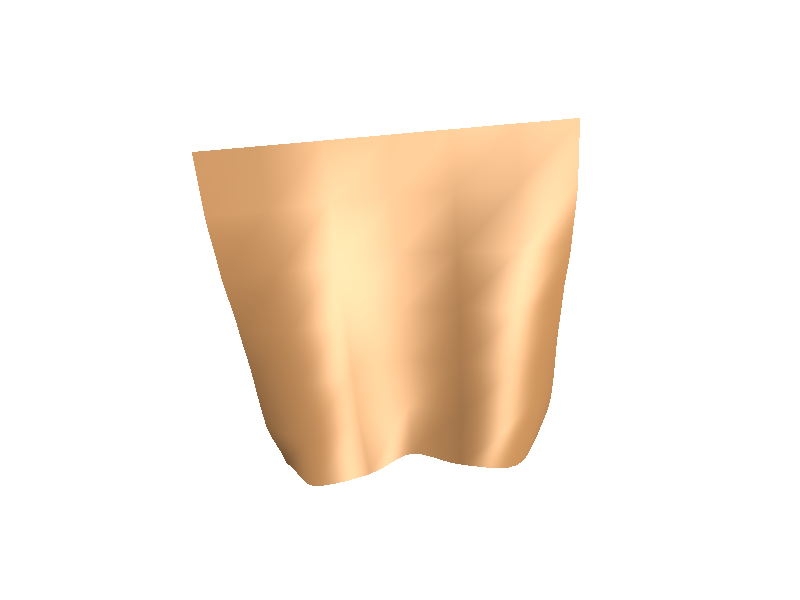
\includegraphics[width=0.5\textwidth]{figures/cloth-surf.png}

    Updating the mesh: $\mathrm{O}(n^2)$ where $n$ is the width of the mesh.

    \begin{center}
      \texttt{python3 cloth.py}
      \hspace{2em}
      \texttt{python3 opengl\_cloth.py}
    \end{center}
    \begin{markups}
      \addmarkup<1->{annotations/forces.pdf}
    \end{markups}
  \end{frame}

  \begin{frame}
    \frametitle{Marching cubes.}
    \framesubtitle{\itshape\bfseries\sffamily demo}

    \centering
    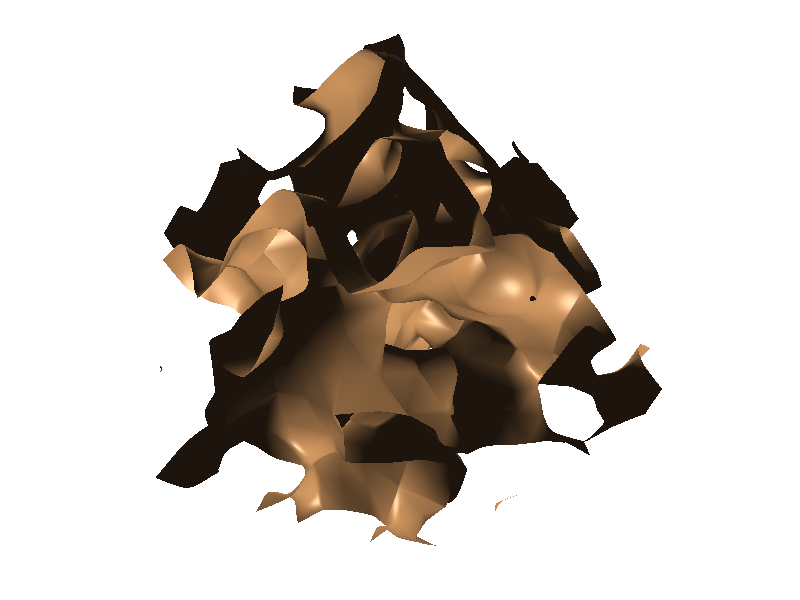
\includegraphics[width=0.5\textwidth]{figures/marching-cubes.png}

    \begin{center}
      \texttt{python3 cubes.py}
      \hspace{2em}
      \texttt{python3 opengl\_cubes.py}
    \end{center}
  \end{frame}

  \Section{Conclusion}

  \begin{frame}
    \frametitle{Limits: continuity.}
    \begin{markups}
      \addmarkup<1>{annotations/discontinuity-mesh.pdf}
      \addmarkup<2>{annotations/discontinuity-curved.pdf}
    \end{markups}
  \end{frame}

  \begin{frame}[standout]
    \itshape\bfseries\LARGE\centering
    Any questions?
  \end{frame}
\end{document}
